\documentclass[12pt, a4paper]{article}
\usepackage[a4paper, bindingoffset=0.2in, %
left=0.5in,right=0.5in,top=0.5in,bottom=0.5in,%
footskip=.25in]{geometry}
\usepackage{graphicx}
\usepackage{amssymb}
\usepackage{amsmath}
\usepackage{hyperref}
\usepackage{physics}

\title{PSet9 Report}
\author{Ali Abolhassanzadeh Mahani}


\begin{document}
	\maketitle
	\section{Theory}
	The problem is to simulate 100 argon atoms in a space. The potential for the interaction of 
	the atoms is the leonard-jones potential as below:
	\begin{equation}
		U_{ij} = 4\epsilon \left(\left(\frac{\sigma}{r_{ij}}\right)^{12} - 
		\left(\frac{\sigma}{r_{ij}}\right)^6\right), \; 
		r_{ij} \equiv \norm{\vec{r}_i - \vec{r}_j}
		\label{eq:leonard_jones}
	\end{equation}

	First, there are some matters we need to clarify before jumping into the code.
	Trying to simulate the Argon atoms using the SI units is impossible. It takes a lot of time and
	space that is unnecessary. In order to solve this problem, we come up with characteristic 
	units for the system. Our parameters are as follows:
	\begin{equation}
		m_{arg} = \dots, \; \sigma = 3.4 \times 10^{-10} (m), \; \epsilon \simeq 
	\end{equation}
	If we make the following changes:
	\begin{equation}
		m \rightarrow \frac{m}{m_{arg}}, \; U \rightarrow \frac{U}{\epsilon}, \; r \rightarrow 
		\frac{r}{\sigma}
	\end{equation}
	then Eq.~\ref{eq:leonard_jones} becomes:
	\begin{equation}
		u_{ij} = 4 \left(\frac{1}{r_{ij}^{12}} - \frac{1}{r_{ij}^6}\right)
	\end{equation}
	
	Using this transformation, the equations for kinetic and potential energy of the system 
	are:
	\begin{equation}
		\begin{aligned}
			K &= \frac{1}{2}\sum_{i=1}^{n} v_i^2,\\
			U &= \sum_{i < j} u_{ij} = \frac{1}{2} \sum_{i, j = 1}^{n} u_{ij}
		\end{aligned}
	\end{equation}

	\section{The MDSystem Class}
	I start by writing a class called \texttt{MDSystem} that takes in the size of the box, the
	number of atoms, and the initial position of the atoms in the box. Then, it assigns a speed 
	according to the temperature of the system and speads the velocities in random directions.
	Then, we make sure that the velocity of the center of mass (CoM)  of the system is zero,
	by calling \texttt{stabilize\_system()}. This is because the notions of temperature is defined 
	in a stationary system in the LAB frame. This is all the work of \texttt{\_\_init\_\_()}
	
	The algorithm for the evolution of the system is the "verlet" method, since it intrinsicly conserves the energy of the system as discussed in the previous homeworks. 
	
	Then, we have the periodic boundary conditions that need to be applied both when a 
	particle is passing through one side of the box, and when we are calculating the interaction 
	of the particles. For the interactions, since the Leonard-Jones interaction is short-range, we
	set a "cutoff radius" from each particle and assume that only the particles within that range 
	can interact with the subjected atom. The value chosen for the cutoff radius is $2.5$ in the 
	characteristic units.
	
	\section{The Simulation}
	\subsection{Analysis}
	\subsubsection{Conservation of Energy and number of atoms}
	First, we check the conservation of energy and the number of particles in the left side of the 
	box. Since our initial setup was to place the atoms in a grid in the left half of the box, we 
	should expect the value to start from total number of atom (in our case 100) and move towards half of that value (50 for our case), and then to oscillate about that value. As for
	energy, we expect it to be conserved since our system is micro-canonical (NVE) as seen in
	Fig~\ref{fig:energy_and_left}
	
	\begin{figure}[h!]
		\centering
		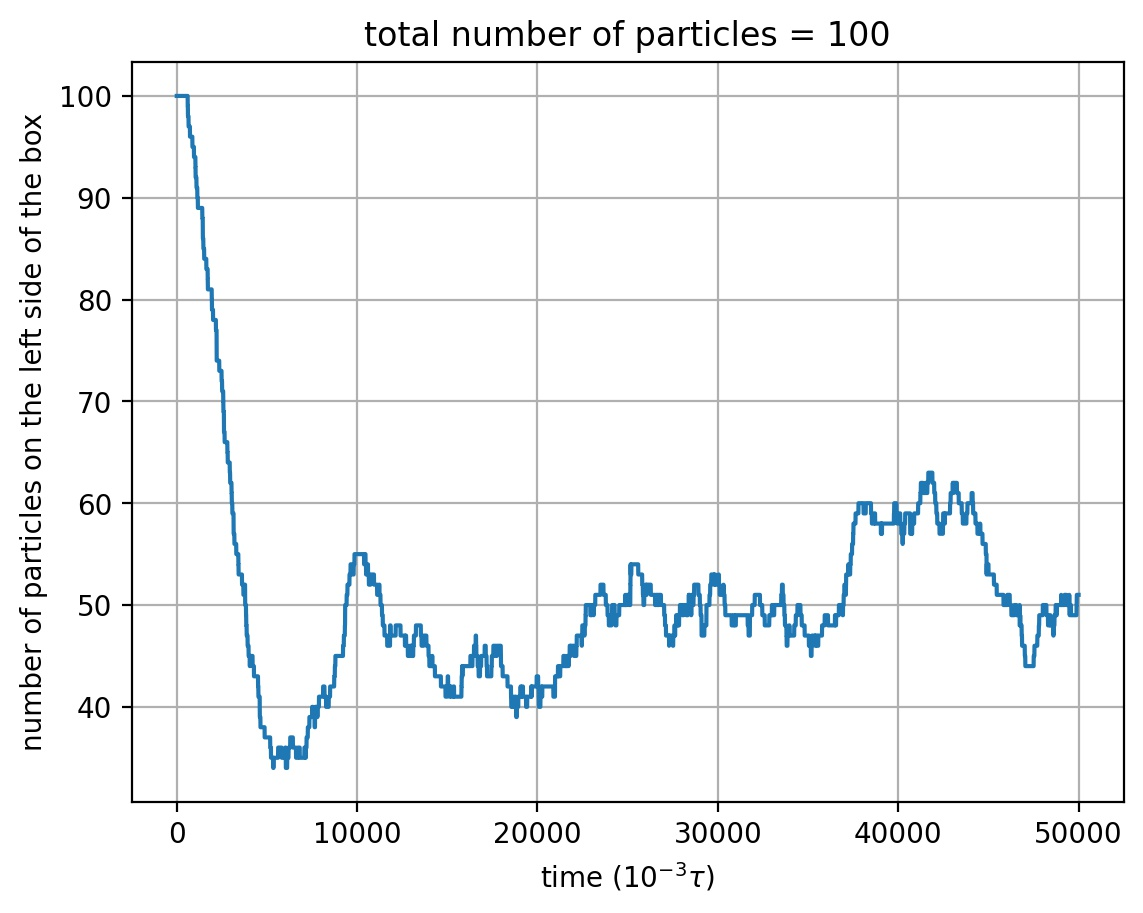
\includegraphics[width=.45\linewidth]{../results/particles_on_left100_50000.jpg}
		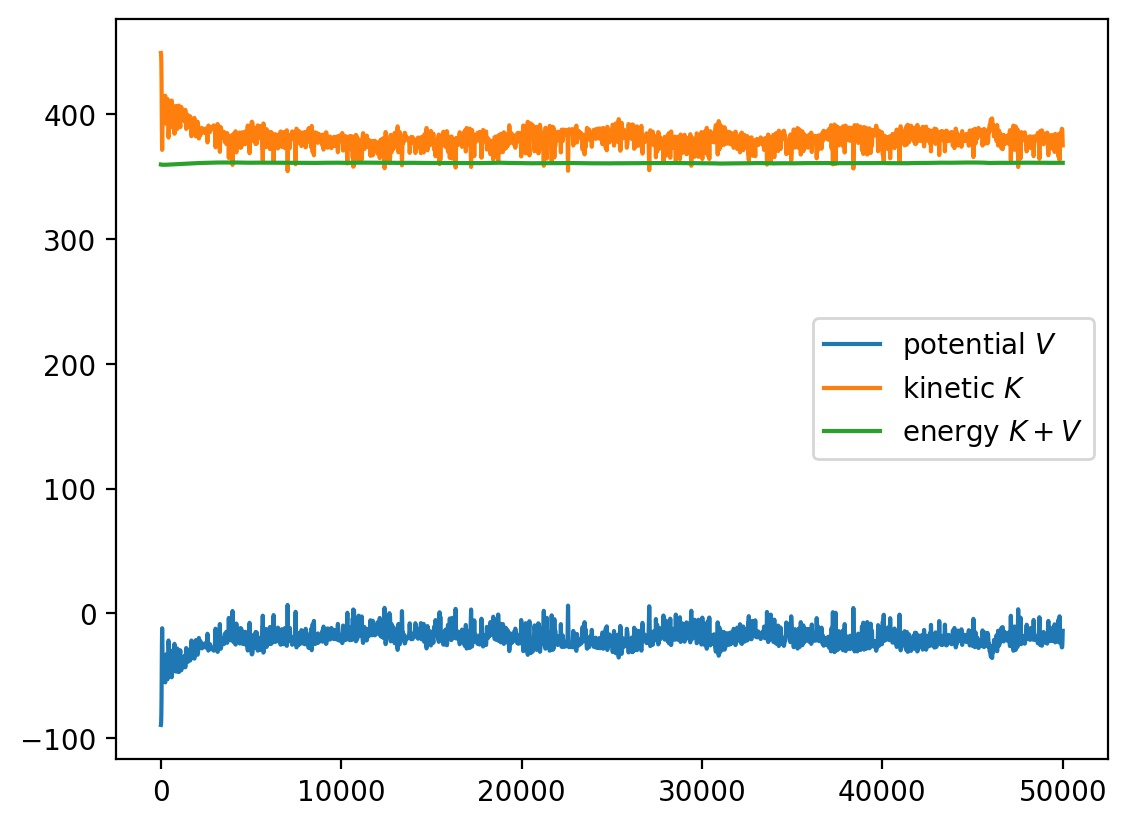
\includegraphics[width=.45\linewidth]{../results/energy_conservation100_50000.jpg}
		\caption{As expected, on the left, we can see that the number of particles on the 
		left side of the box reaches, and oscillates about half of the atoms. And on the right, we
		can clearly witness the conservation of energy}
		\label{fig:energy_and_left}
	\end{figure}

	\subsubsection{Temperature, Pressure, and equilibrium}
	Now, we turn our heads to a thermodynamic observable, temperature. The thermodynamic 
	equation for temperature is:
	\begin{equation}
		\frac{1}{2} \sum_{i}^{N}\sum_{e} v_{ie}^2 = Nd \frac{1}{2}k_B T
	\end{equation}
	where $N$ is the number of particles, $d$ is the dimension of the system (in our case 2) and 
	T, the temperature. In the system that $k_B$ is $1$, we can rewrite the equation as follows:
	\begin{equation}
		\sum_{i}^{N} \sum_{e} v_{ie}^2 = N d T
	\end{equation}
	one should take note that in our case, we used a convention, namely that the system is 
	stabilized (i.e., the CoM velocity is zero). In Thermodynamics this doesn't matter due to the 
	size of our ensemble, but in MD it matters. So we have:
	\begin{equation*}
		N d T \rightarrow (N-1) d T
	\end{equation*}
	
	
	
	
	
\end{document}